\documentclass[11pt]{article}
\usepackage{graphicx}
\usepackage{amsmath}
\usepackage{booktabs}
\usepackage{geometry}
\usepackage{hyperref}
\usepackage{float}
\usepackage{setspace}
\geometry{margin=1in}
\setlength{\parindent}{0pt}

\begin{document}

\begin{center}
    \vspace*{0.5cm}
    {\Huge\bfseries Earnings Case Study\par}
    \vspace{0.8cm}
    {\large Nathan Brown\par}
    {\large \today\par}
    \vspace{1cm}
\end{center}

\tableofcontents
\newpage

\section{Duolingo: DUOL}
    \subsection{2023-02-28 Earnings Report}
        \begin{itemize}
            \item \textit{Earnings Summary:} DUOL reported sixth consecutive quarter of user/growth acceleration with DAUs +62\% YoY to 16.3M and MAUs +43\% to 60.7M. Other key KPIs (total revenues, adjusted EBITDA, paid subscriber count) all increased by 40\%+, soothing worries about profitability saturation.
            \item \textit{Price Action:} Sideways price action following uptick in growth from early 2023. Earnings report led to heavy 22\% spike (on next trading day) with heavy (4x) volume followed by consistent gains over the next several weeks. DUOL also announced two weeks later (on Mar 14) that ``Duolingo Max'' would be powered by GPT-4. This captured AI hype and led to a further up-and-to-the-right movement. See Figure 1.
            \begin{figure}[h]
                \centering
                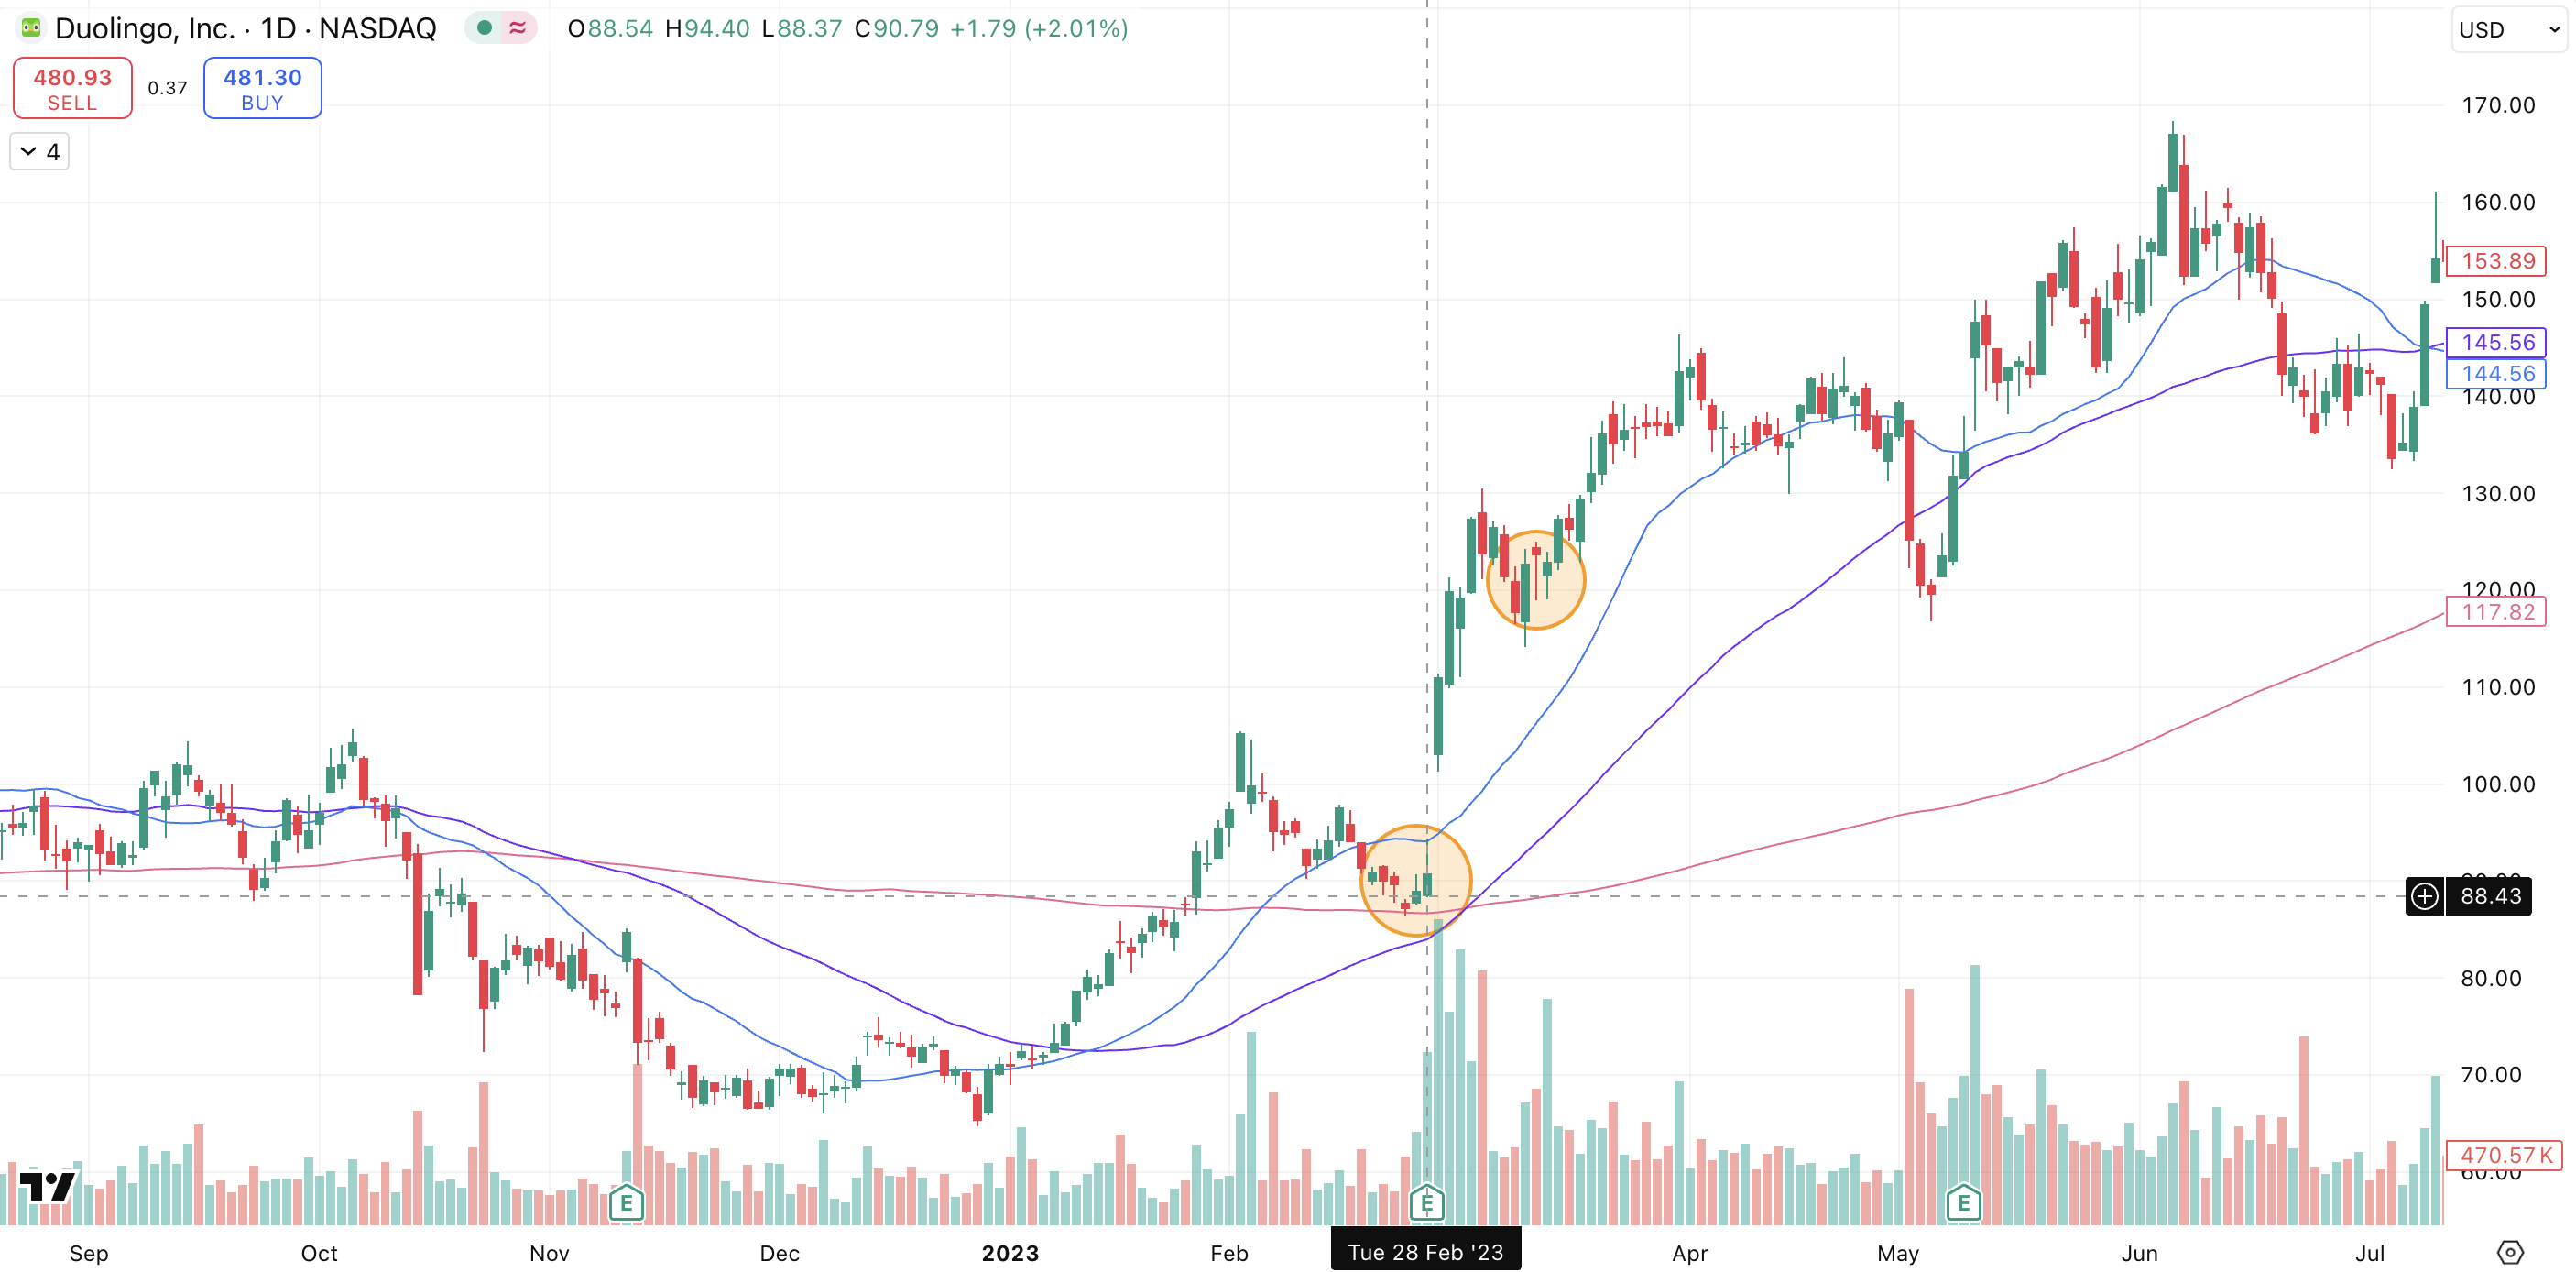
\includegraphics[width=0.8\linewidth]{images/DUOL1.png}
                \caption{1st circle indicates earnings report, 2nd circle indicates AI announcement}
            \end{figure}
        \end{itemize}
    \subsection{2025-05-01 Earnings Report}
        \begin{itemize}
            \item \textit{Earnings Summary:} Duolingo posted another strong quarter, with GAAP EPS of \$0.72 beating consensus by 20¢ and revenue climbing to \$231M (+4\% vs. Street). It marked the company’s first-ever 10M+ paid subscriber quarter (10.3M, +40\% Y/Y), as the freemium-to-paid funnel remained robust. User growth reaccelerated once again — DAUs rose 49\% Y/Y to 46.6M, and the DAU/MAU ratio improved to 35.8\%, pointing to higher engagement and retention. Adj. EBITDA margin expanded 900 bps Y/Y to 27\%, with free cash flow margin at 24\%. Management also raised full-year revenue guidance and signaled continued operating leverage, easing concerns about cost pressures tied to AI investments.
            \item \textit{Price Action:} Shares spiked over 20\% on high volume following the print. The rally came on elevated volume and was supported by a flurry of analyst upgrades and bullish headlines calling Duolingo a “consumer-AI showcase.” Investors appeared encouraged by traction in Duolingo Max, ongoing AI content scaling, and strong user/subscriber trends despite tough comps. The stock continued drifting upward in the days that followed, fueled by optimism around new product verticals and gross margin expansion potential. See Figure 2.
            \begin{figure}[h]
                \centering 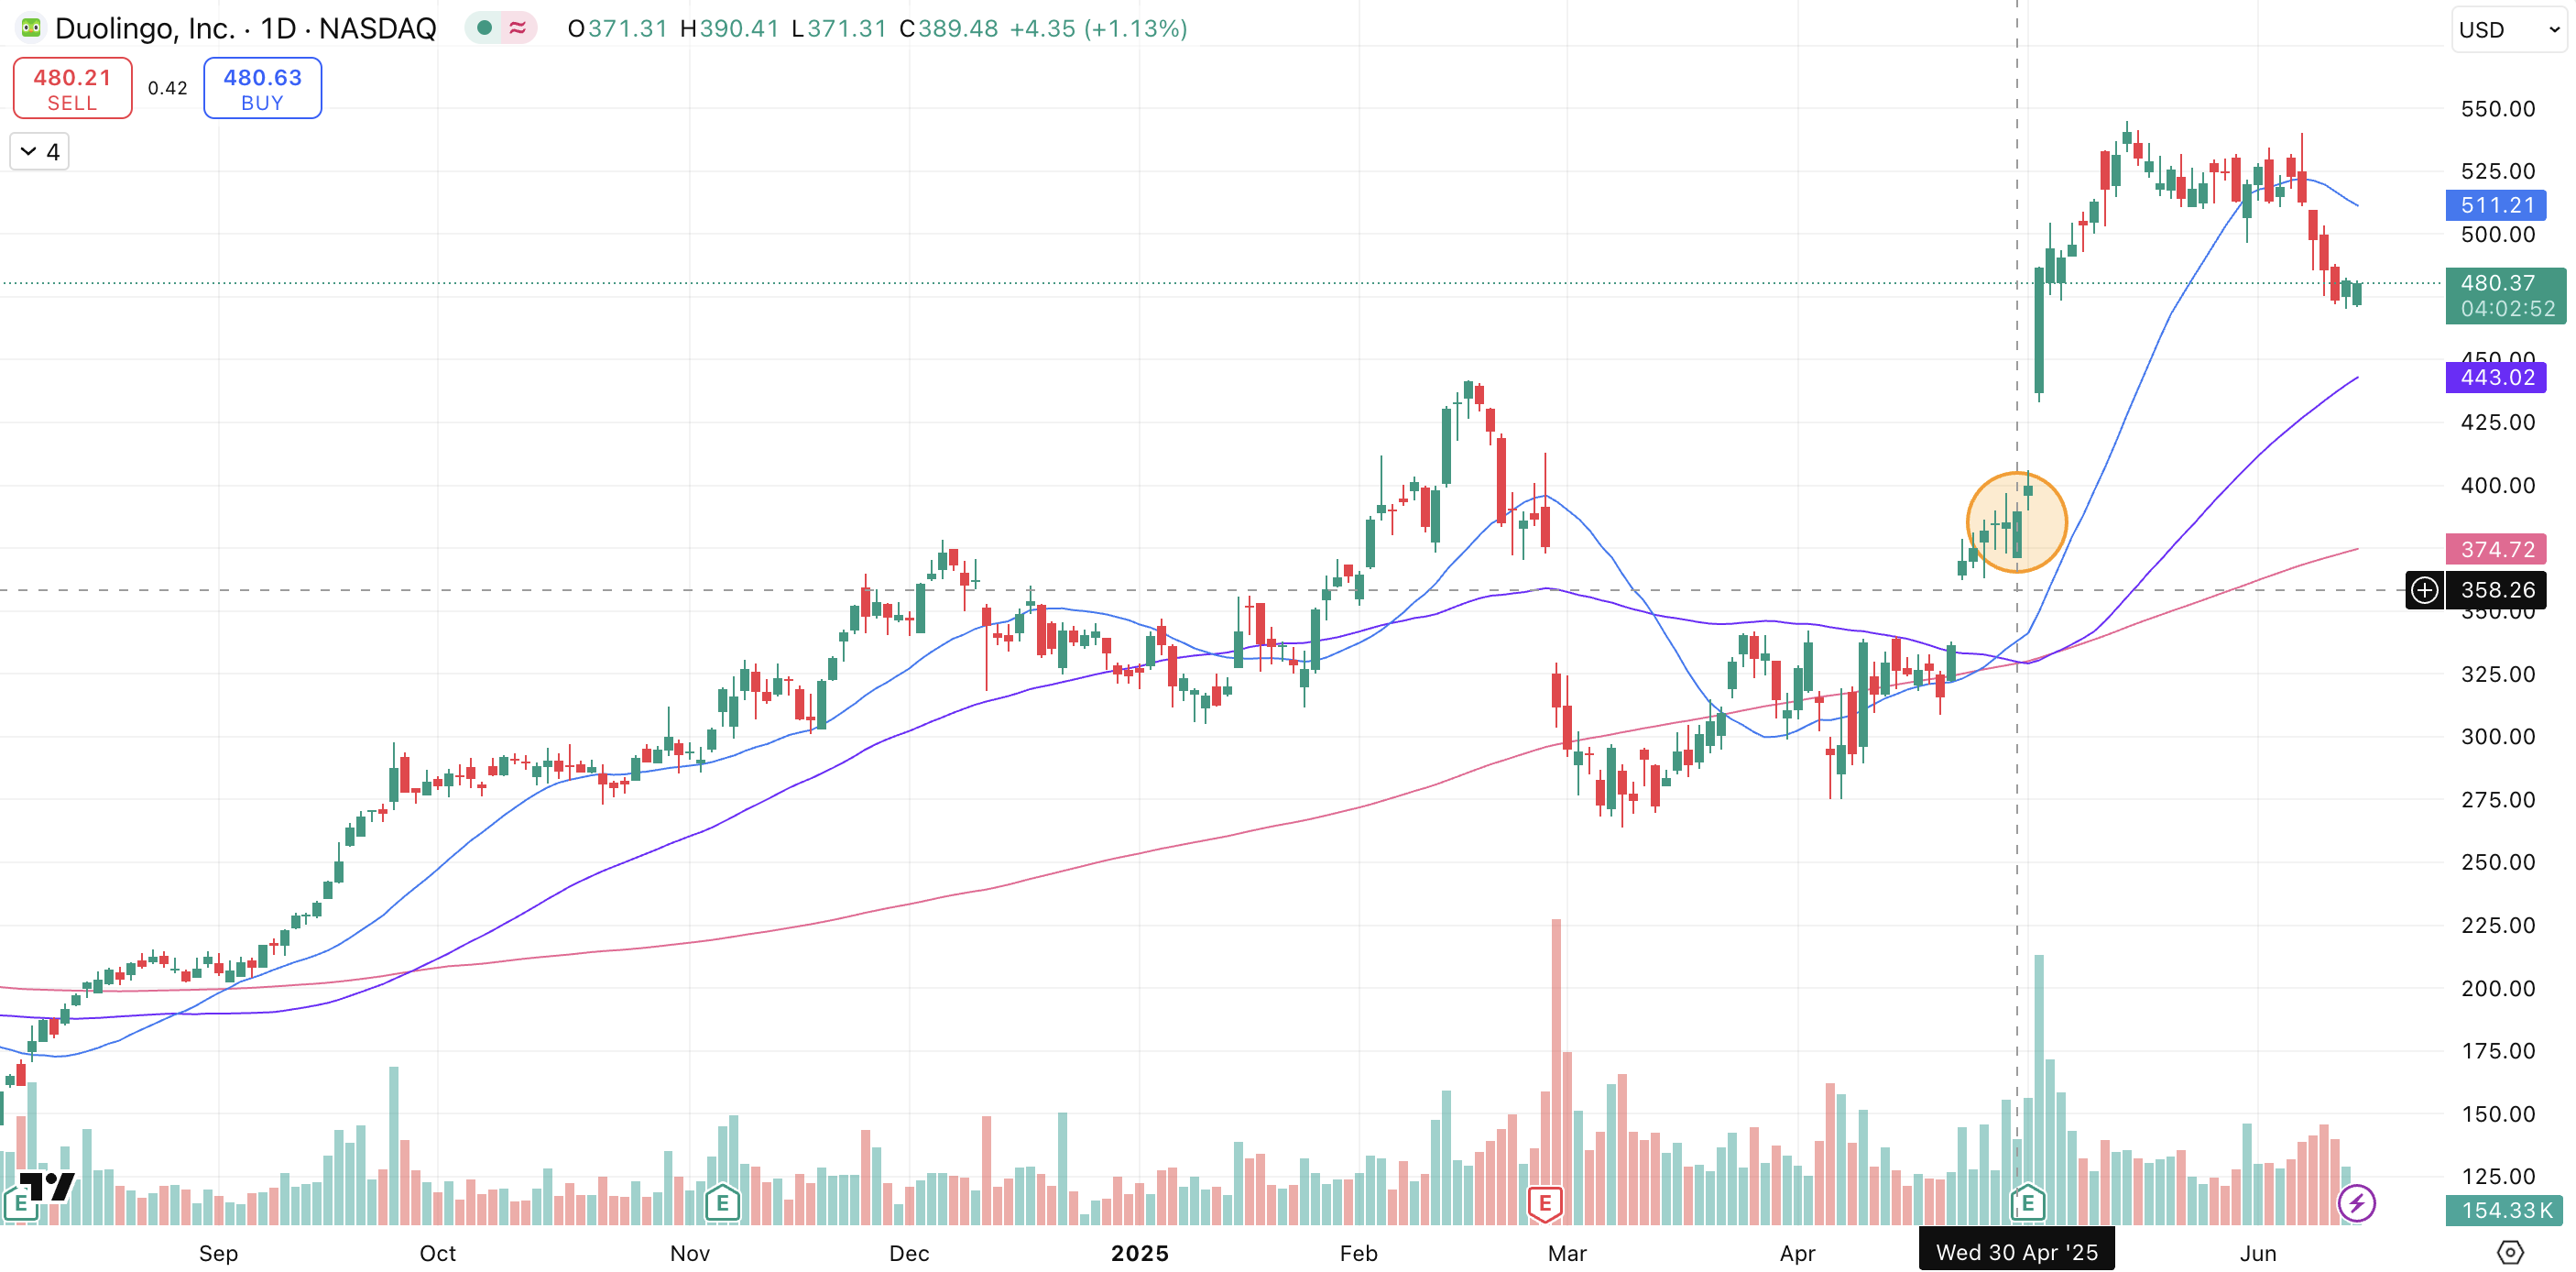
\includegraphics[width=0.8\linewidth]{images/DUOL2.png}
                \caption{Stock surged post-earnings on stronger-than-expected results and bullish guidance.}
            \end{figure}
        \end{itemize}
    \subsection{Pattern}
        The stock rallied on a rare combination of strong, consistent user and subscriber growth, expanding margins, and clear progress in AI integration—notably with Duolingo Max and AI-driven content creation—which reinforced confidence in both near-term execution and long-term scalability.  \section{Intuitive Machines: LUNR}
    \subsection{2024-02-15 Moon Mission Spike}
        \begin{itemize}
            \item \textit{Cause of Breakout:} NASA and Intuitive Machines gave a formal ``GO'' for launch on Feb 12 for LUNR's IM-1 ``Odysseus'' lunar-lander mission. On Feb 15, Falcon 9 successfully launched IM-1, the first US attempt to soft-land on the moon in 52 years. This drew heavy mainstream \& social media coverage and led to a high volume breakout and an $>$30\% increase in the stock price in early-market.
            \item \textit{Subsequent Price Action:} The party did not last long. On Feb 22, \textit{Odyseuss} landed sideways and the CEO reported that some of the instruments were not working properly. Investor sentiment dropped significantly, which triggered day traders to unwind their positions, short sellers to re-enter and the price to drop back to \$6 within a couple of days. See Figure 3.
            \begin{figure}[h]
                \centering 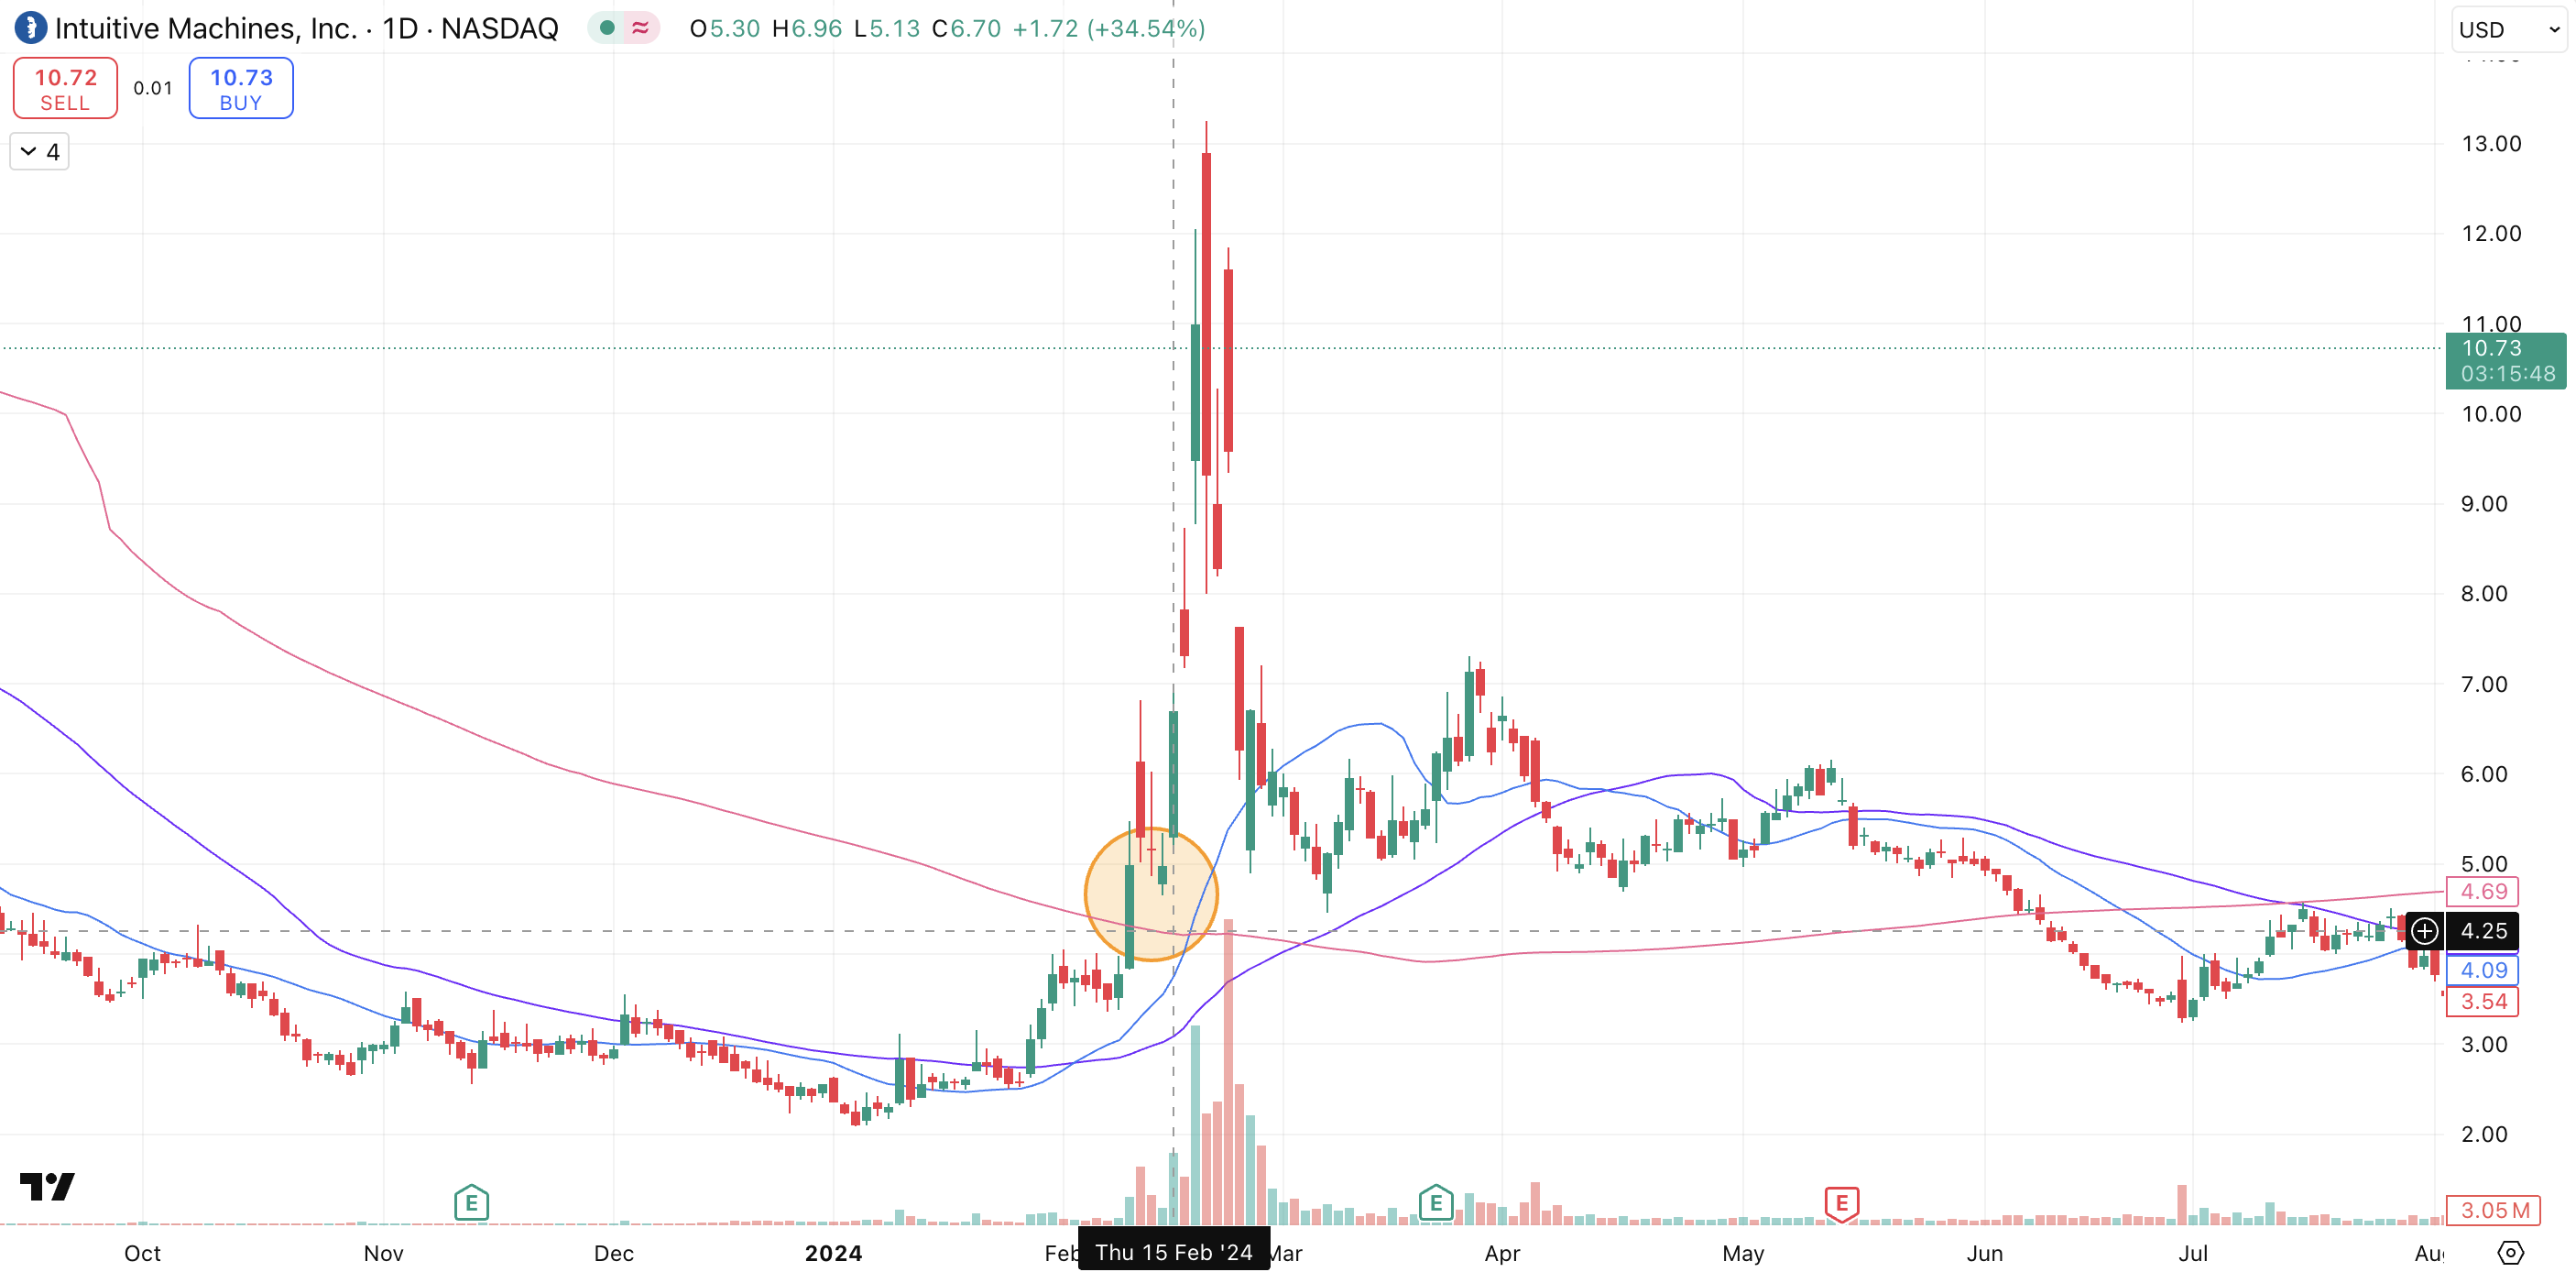
\includegraphics[width=0.8\linewidth]{images/LUNR1.png}
                \caption{The spike and following decline illustrates the volatility of space-based companies whose stock price is heavily influenced by mission results.}
            \end{figure}
        \end{itemize}
    \subsection{2024-11-14 Earnings Report}
        \begin{itemize}
            \item \textit{Earnings Summary:} EPS missed heavily: -\$0.82 EPS vs. -\$0.12 EPS est. However, the stock jumped heavily due to a couple of factors: (1) record funded backlog of \$316.2m; (2) awarded \$117m contract through NASA's Commercial Lunar Payload Services (CLPS) initiative; (3) only company to be awarded Near Space Network (NSN) contract from NASA with max potential value of \$4.82B. The company also achieved record revenues in Q3, up 359\% YoY.
            \item \textit{Subsequent Price Action:} The price fell 13\% on the day the earnings report occurred on, likely due to negative investor sentiment on the huge EPS failure. However, the price quickly corrected +21\% the next day and continued its up-and-to-the-right pattern for the next 1-2 weeks. See Figure 4.
            \begin{figure}[h]
                \centering 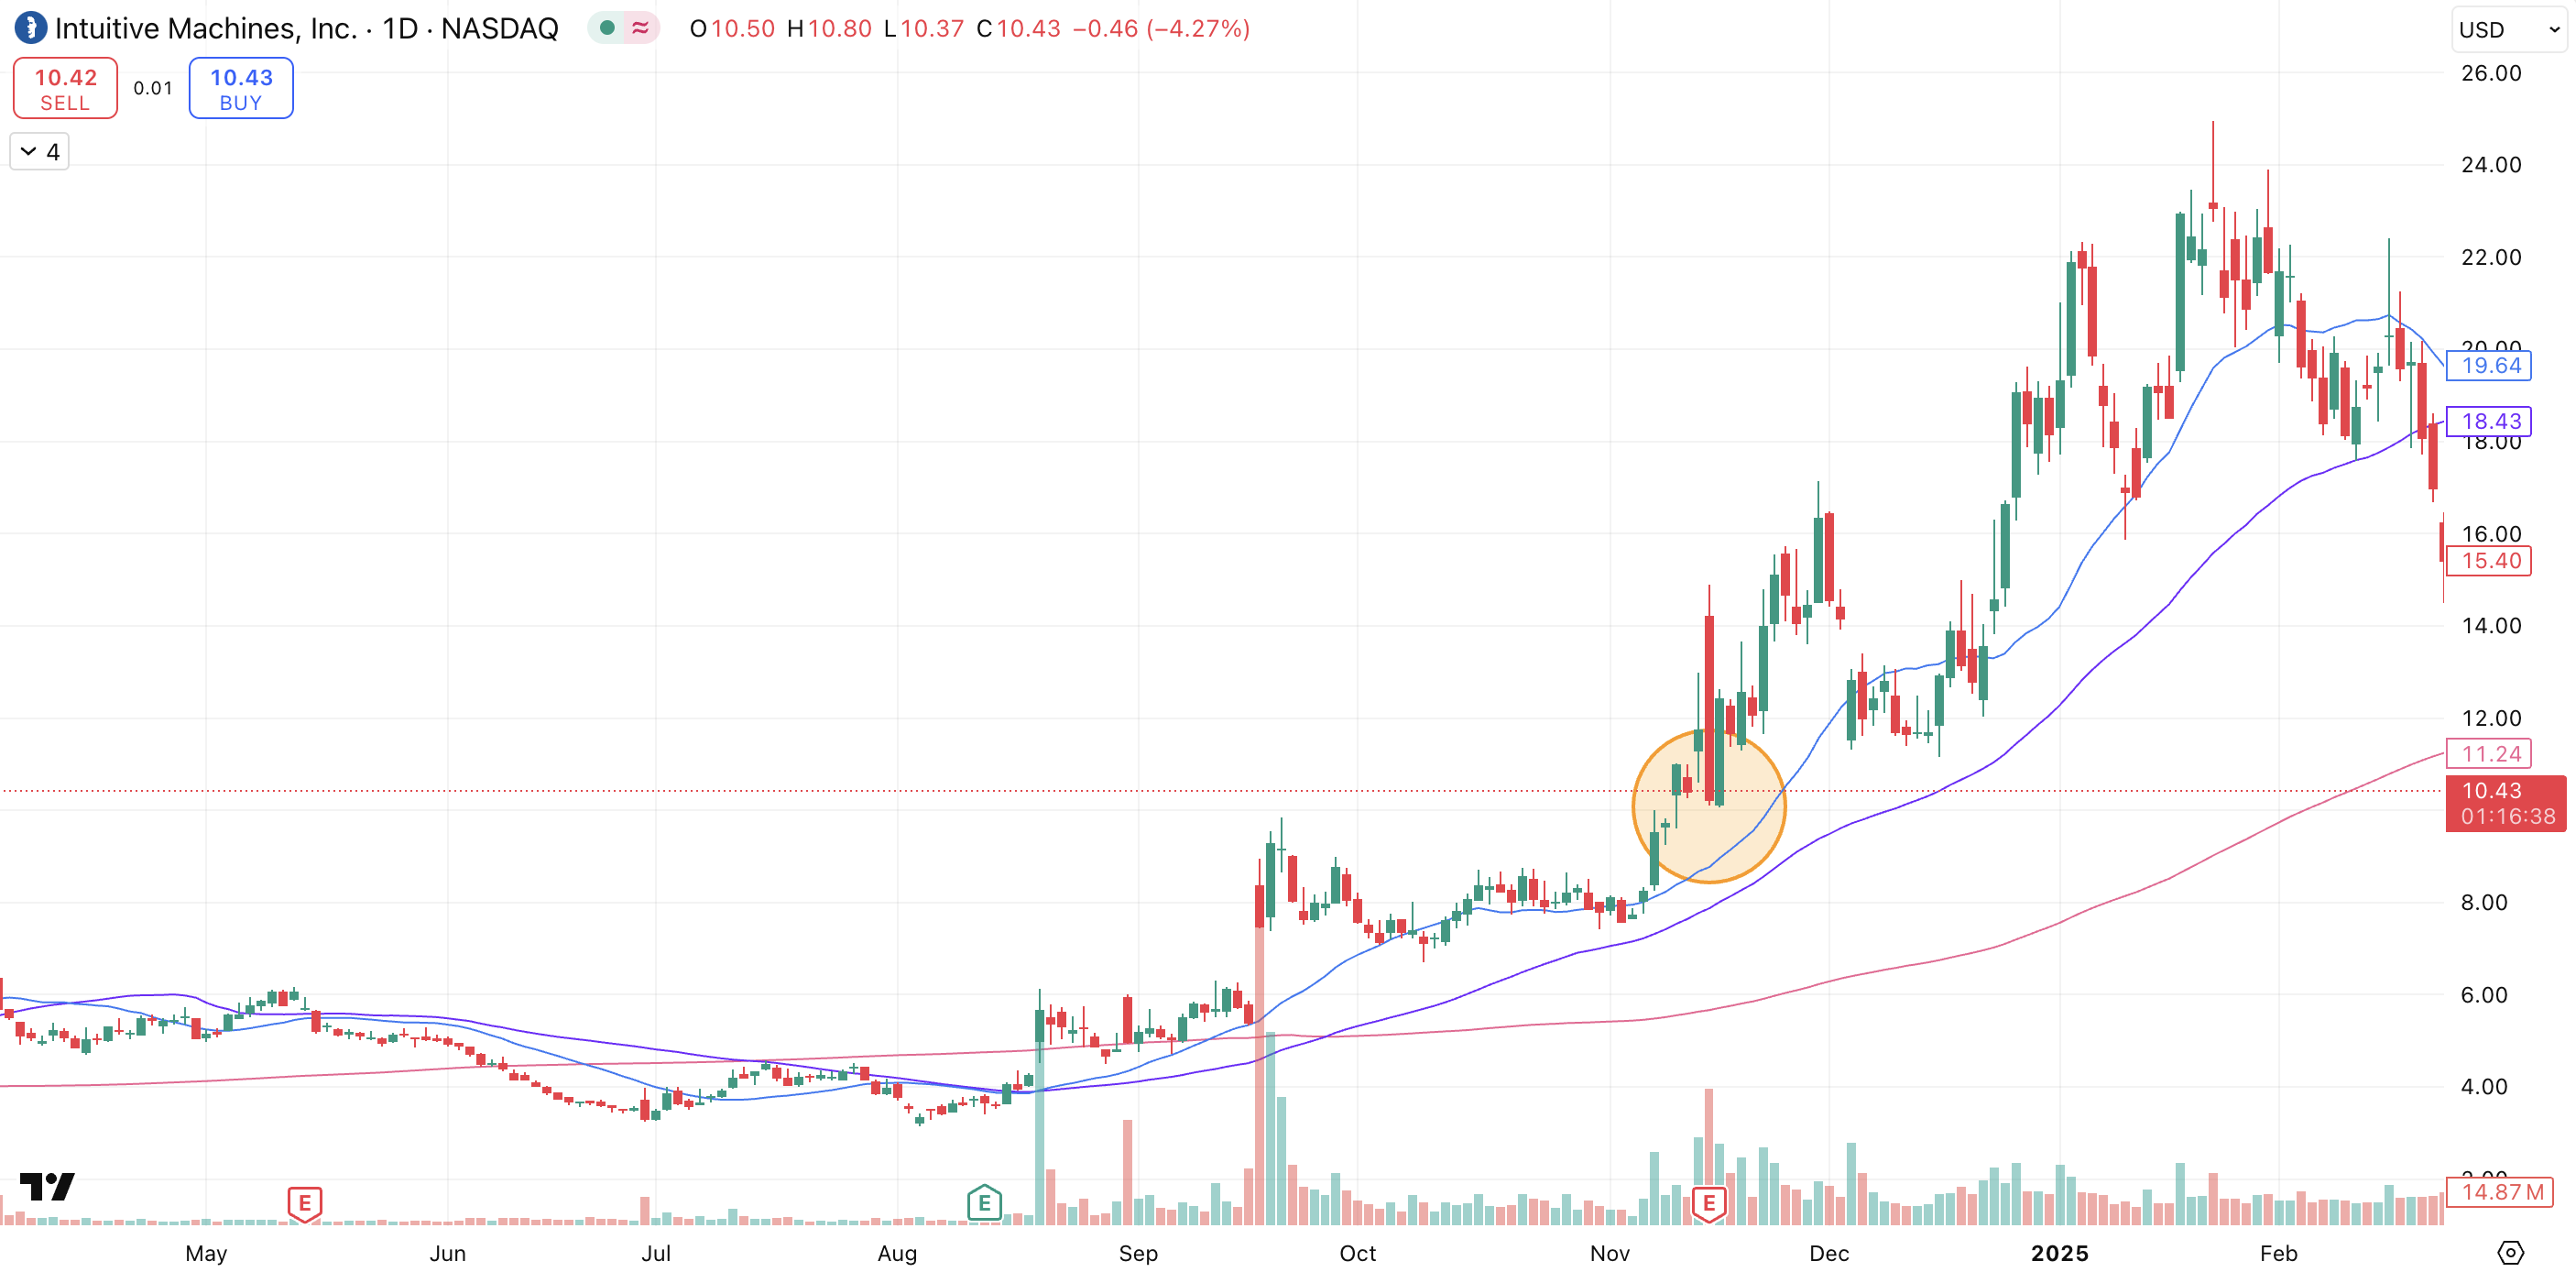
\includegraphics[width=0.8\linewidth]{images/LUNR2.png}
                \caption{Earnings reports don't always predict price action.}
            \end{figure}
        \end{itemize}
        \subsection{Pattern}
        LUNR’s stock tends to overreact to milestone headlines—both positive and negative—with follow-through largely dependent on perceived execution and media narrative. Sharp post-event corrections suggest a high degree of speculative trading and little guidance based on fundamentals.
\section{Shopify: SHOP}
    \subsection{2019-04-30 Earnings Report} 
        \begin{itemize}
            \item \textit{Earnings Summary:} Huge beat-and-raise quarter. Q1 revenue was \$320.5m, up 50\% YoY. Adjusted operating income swung to a \$10m profit (expectation was a loss). Adoption of Shopify shipping climbed to 40\% of eligible merchants using Shopify Shipping in the quarter. Management teased new multi-currency and AR launches ahead of a conference in May.
            \item \textit{Subsequent Price Action:} Stock spiked 7\% with 3-4x volume on Apr 30, 2019, added 15\% by week-end, and rallied to close to 40\% by mid-June as investors became interested in high-growth cloud names. See Figure 5.
            \begin{figure}[h]
                \centering 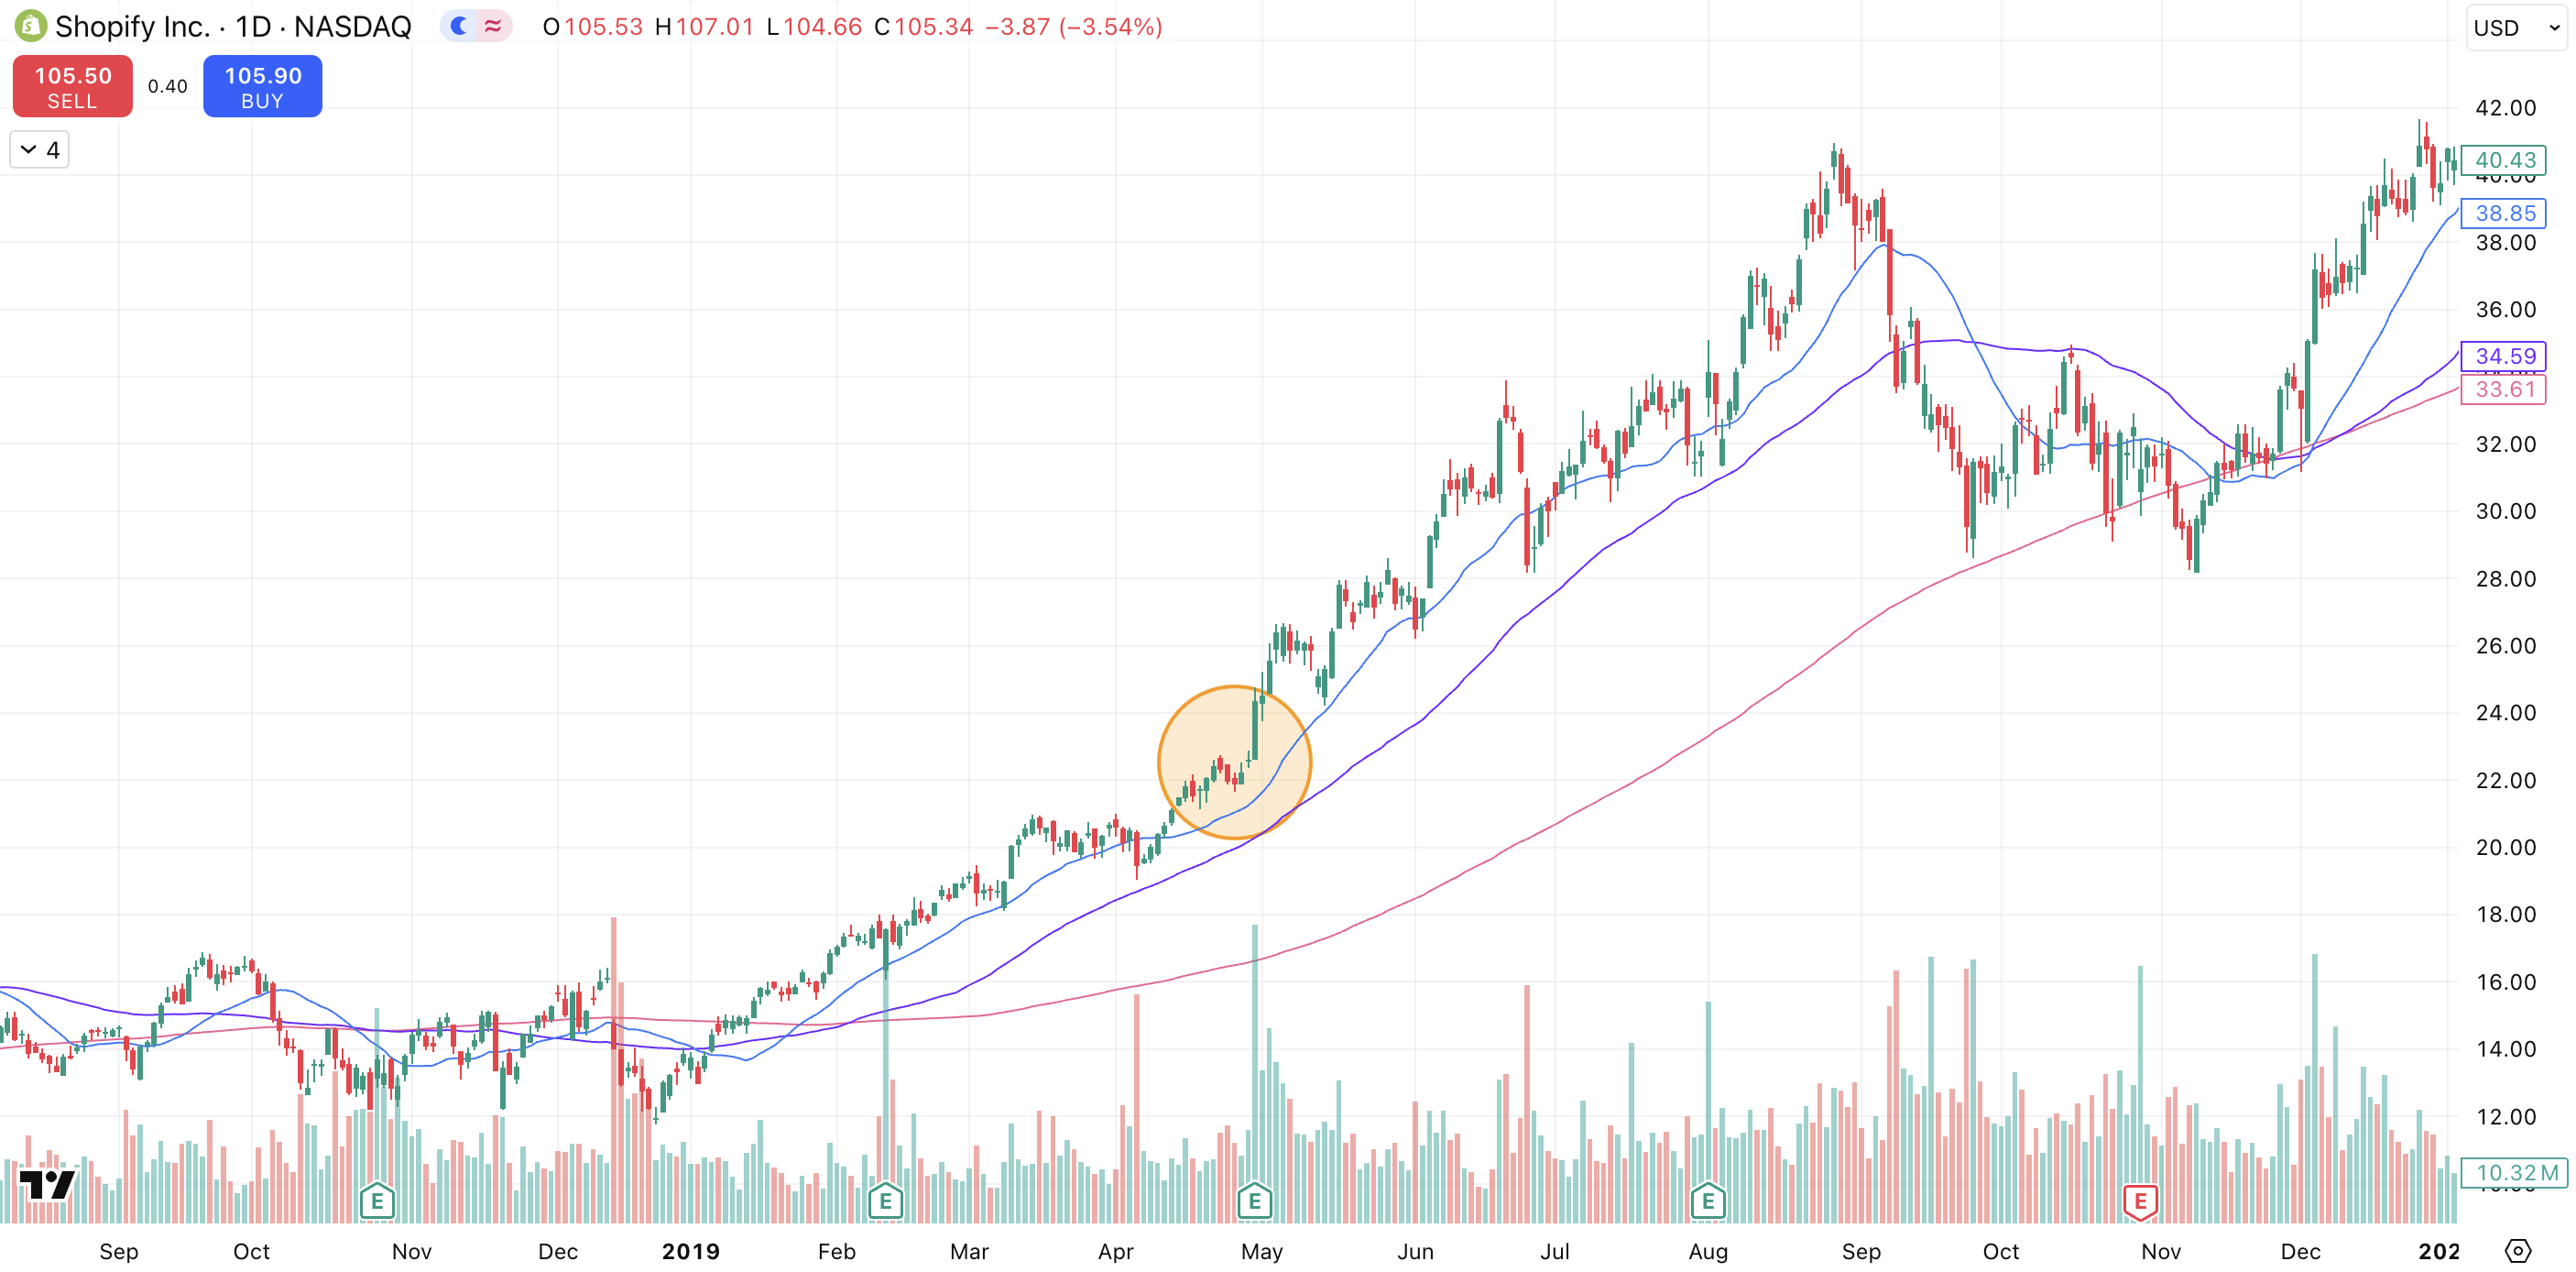
\includegraphics[width=0.8\linewidth]{images/SHOP1.png}
                \caption{While the earnings report did not usher in a dramatic, immediate breakout, it set into motion a consistent series of gains.}
            \end{figure}
        \end{itemize}
    \subsection{2023-11-02 Earnings Report} 
        \begin{itemize}
            \item \textit{Earnings Summary:} Big surprise on adjusted EPS: \$0.24 real vs. \$0.15 expected. Fourth straight positive-FCF quarter. Shopify reiterated long-term 20\%+ FCF margin goal, which reinforced a ``growth + profitability'' narrative. Shopify's guidance for the fourth quarter (forecasting rev. growth in high teens) also encouraged investors, especially since Q4 is the seasonally strongest quarter of the year for SHOP.
            \item \textit{Subsequent Price Action:} Shares lept 22\%---from \$51 to \$63---on Nov 2 on 3x volume and reversed the previous downtrend. As investors rotated into consistently profitable SaaS companies, the price reached \$80 by the end of 2023. See Figure 6.
            \begin{figure}[h]
                \centering 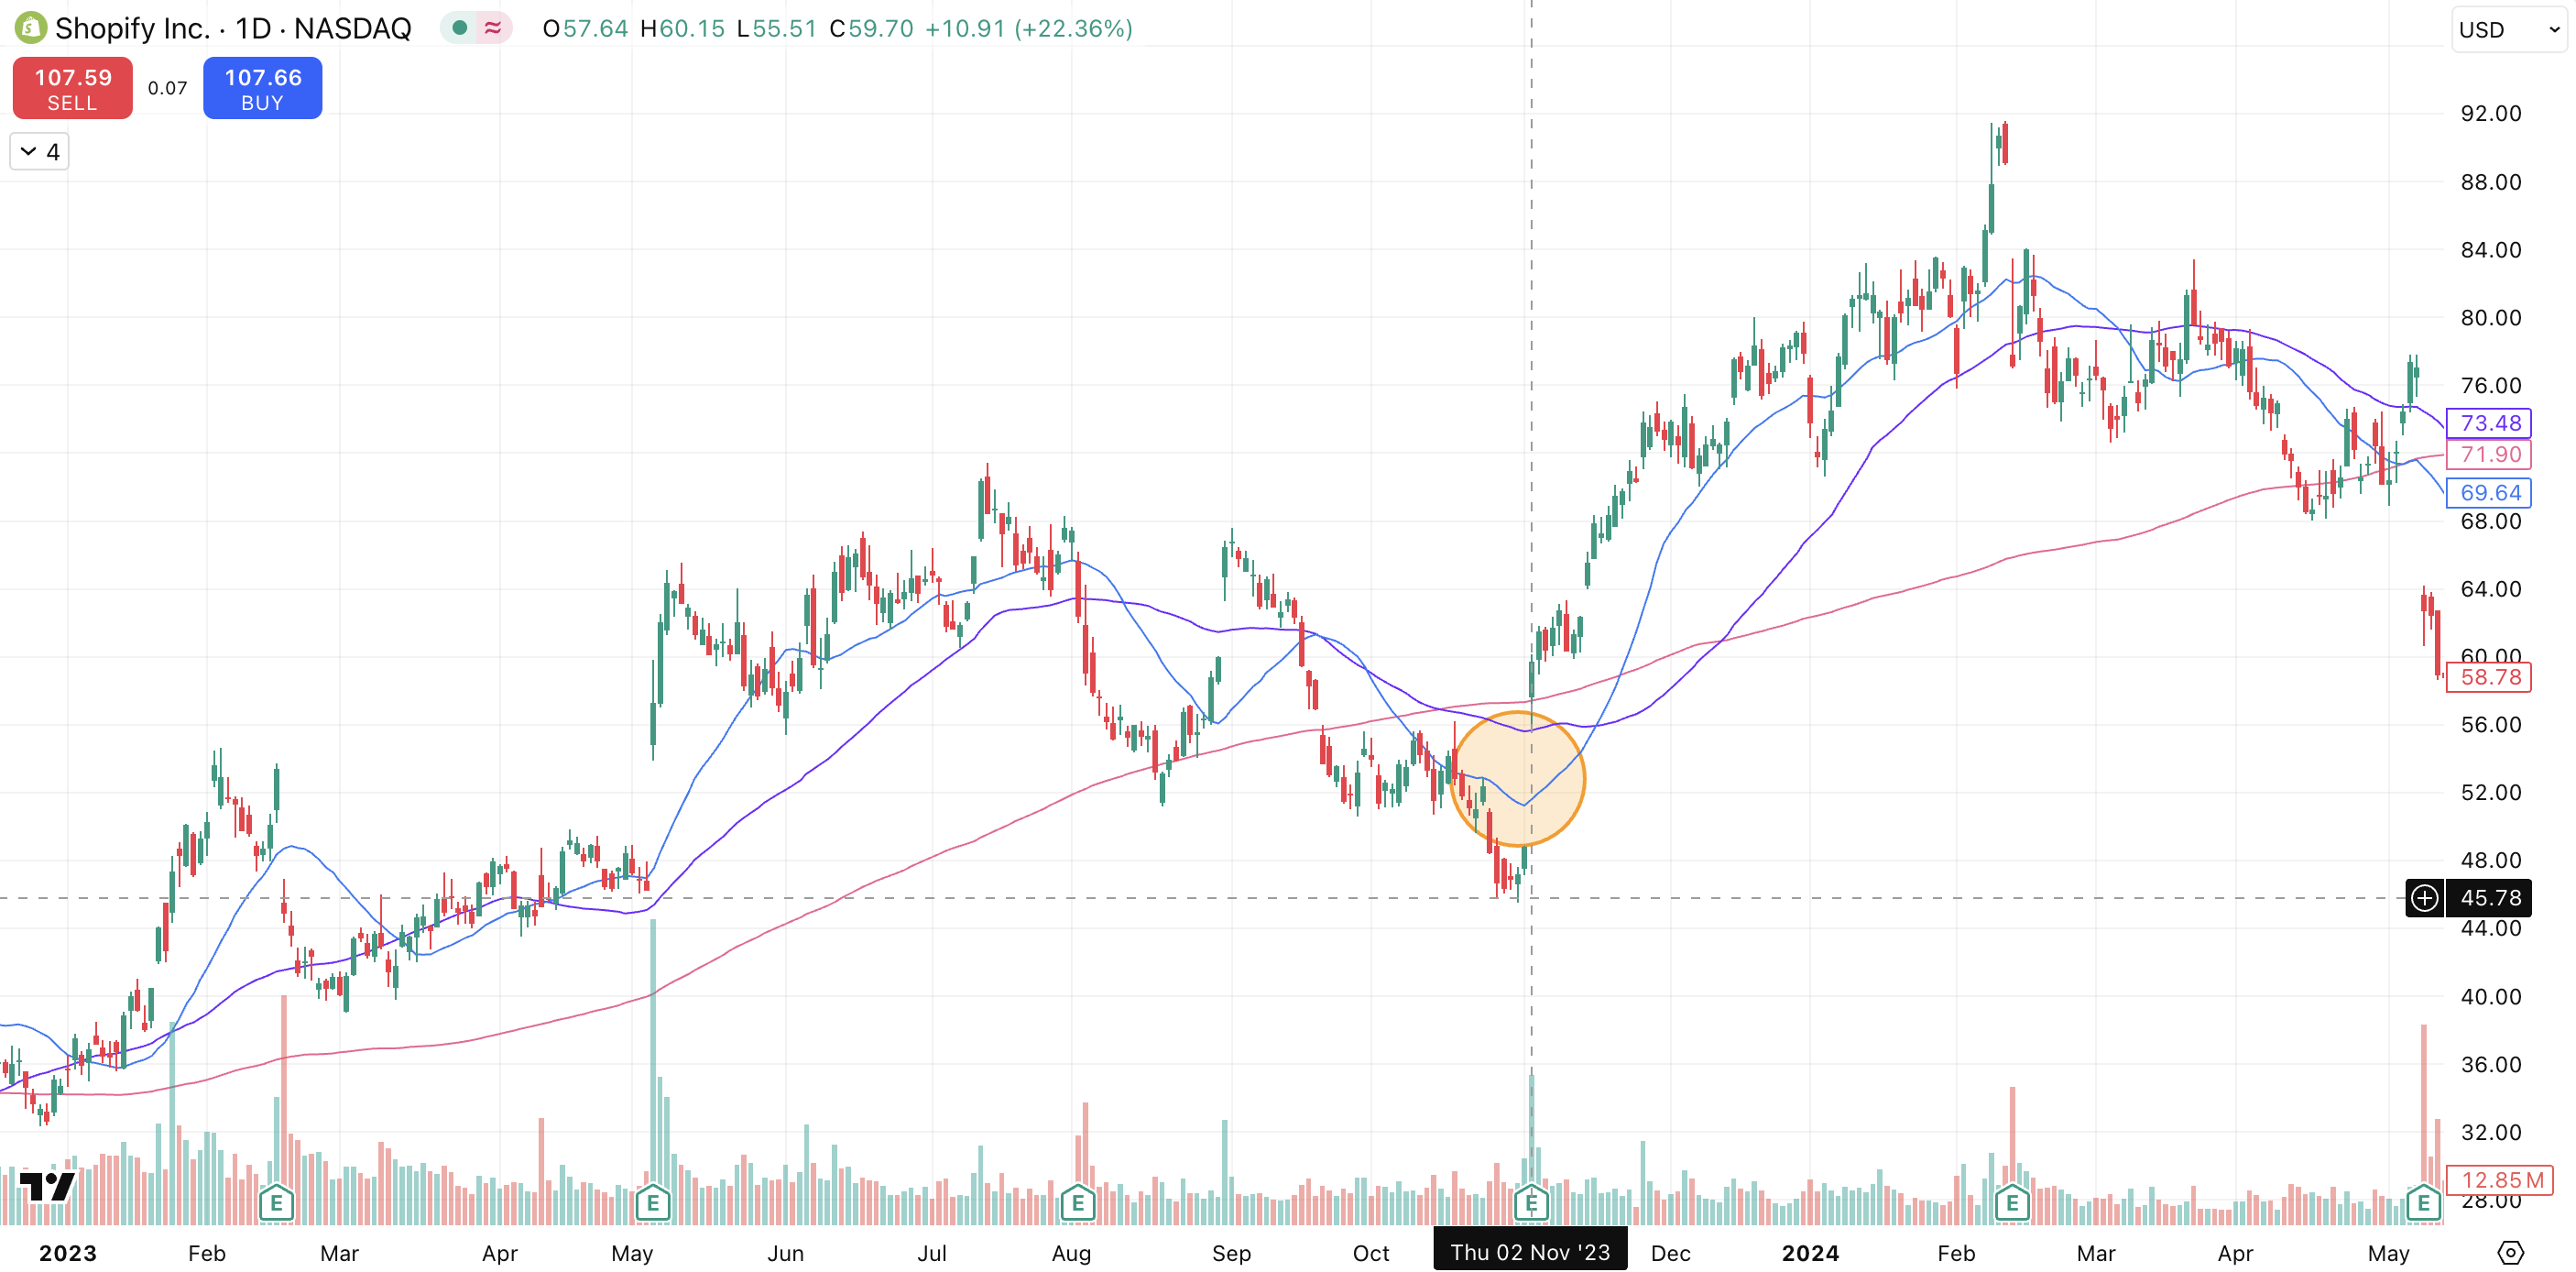
\includegraphics[width=0.8\linewidth]{images/SHOP2.png}
                \caption{Pretty strong reversal of the previous stagnant/negative pattern.}
            \end{figure}
        \end{itemize}
    \subsection{Pattern}
        SHOP thrives on ``beat \& raises'' on the two main things that matter most: revenue growth and free cash flow. Narrative upgrades and macro tailwinds also have helped Shopify during this stage, where tech stocks tend to do very well.
\section{Dave Inc: DAVE}
    \subsection{2024-11-12 Earnings Report}
        \begin{itemize}
            \item \textit{Earnings Summary:} The biggest surprise was operating revenue = \$92.5m, up 41\% YoY, as a fourth consecutive acceleration (16\% $\rightarrow$ 23\% $\rightarrow$ 25\% $\rightarrow$ 31\% $\rightarrow$ 41\%). GAAP net income also was \$0.5m vs. -\$12m in Q3 2023. Average 28-day delinquency rate improved 64 basis points to 1.78\%. Additionally, DAVE had an FTC settlement pending that they settled for \$7m, which eliminated concerns about legal overhang.
            \item \textit{Subsequent Price Action:} The price jumped 44\% on the day, on extremely high 8-10x volume, after the earnings report (which was released after-hours on Nov 12). There was heavy short interest prior to the earnings report, and so shorts raced to cover their positions, which contributed to the high intraday spike. See Figure 7.
            \begin{figure}[h]
                \centering 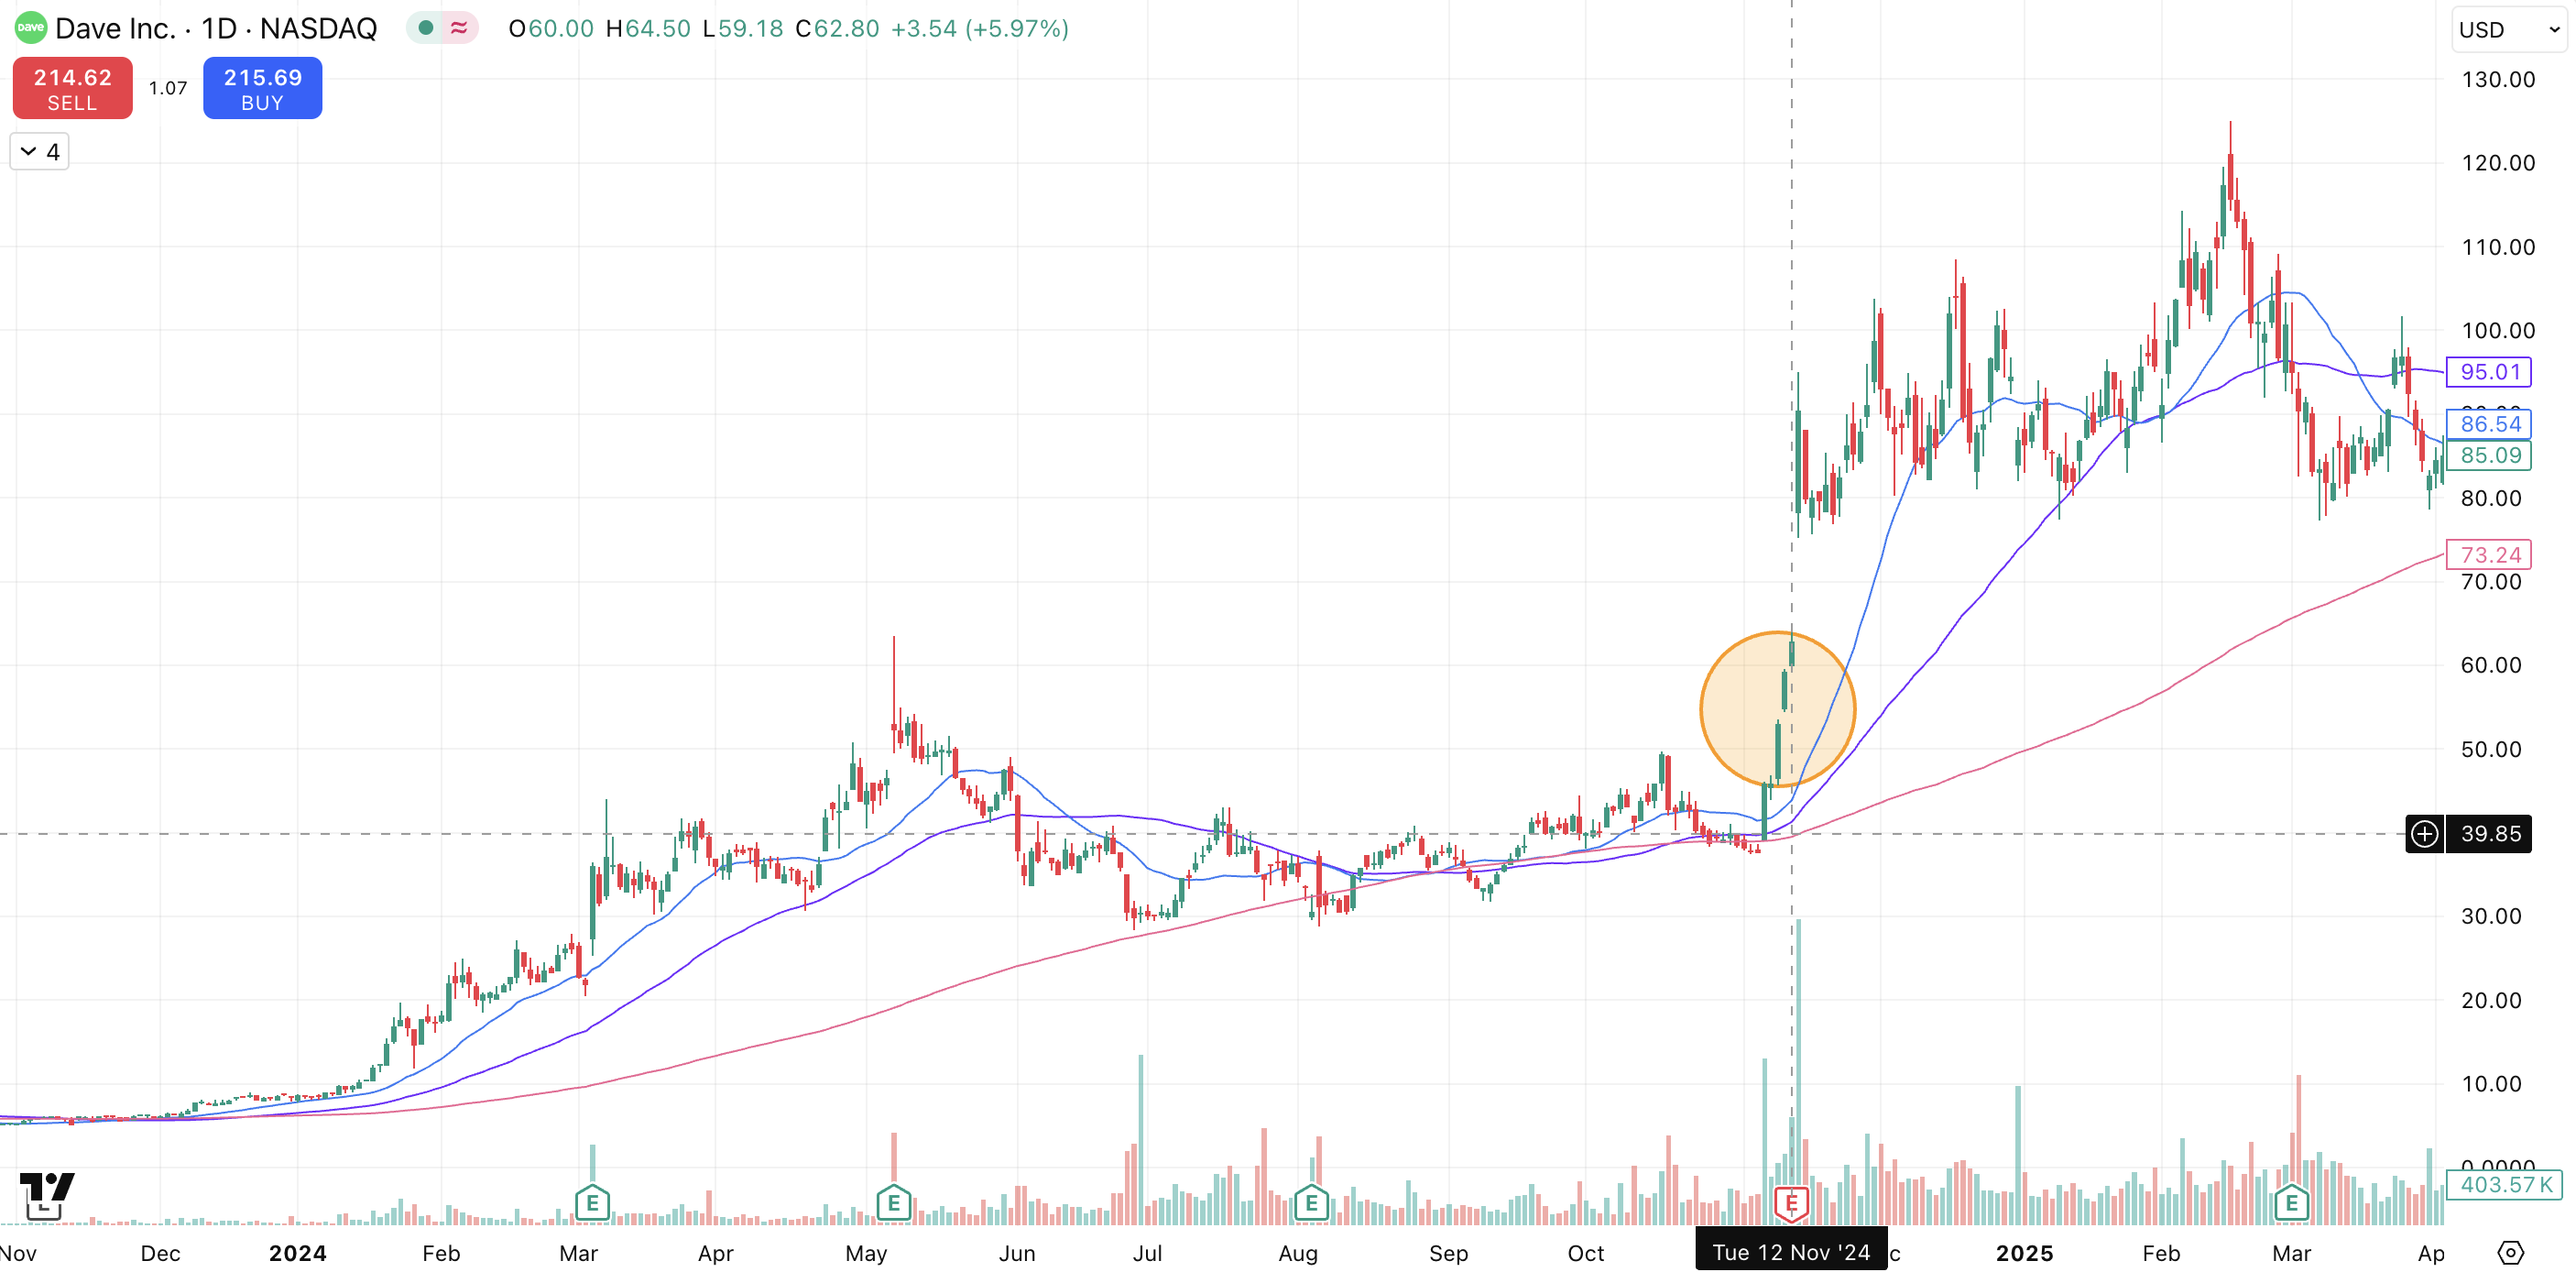
\includegraphics[width=0.8\linewidth]{images/DAVE1.png}
                \caption{Large spike. Interestingly, did not usher in much of a consistent up-and-to-the-right movement, indicating relative investor uncertainty.}
            \end{figure}
        \end{itemize}
    \subsection{2025-05-08 Earnings Report}
        \begin{itemize}
            \item \textit{Earnings Summary:} Crazy beats on every line. \$1.97 EPS vs estimated \$0.764 EPS. Net profit of \$28.8m vs. -\$2m expected. \$50m share-buyback approved by management, which accounted for 20\% of float. All metrics said ``GO'' and management gave drastically higher guides for revenue and EBITDA.
            \item \textit{Subsequent Price Action:} 30\% of shares were held short. Insane positive numbers triggered an extremely violent short squeeze on 10x volume. In two days, price jumped from \$107 to \$167. Fintech peers also rallied at the time due to anticipated rate cuts, providing a positive macro environment for DAVE. See Figure 8.
            \begin{figure}[h]
                \centering 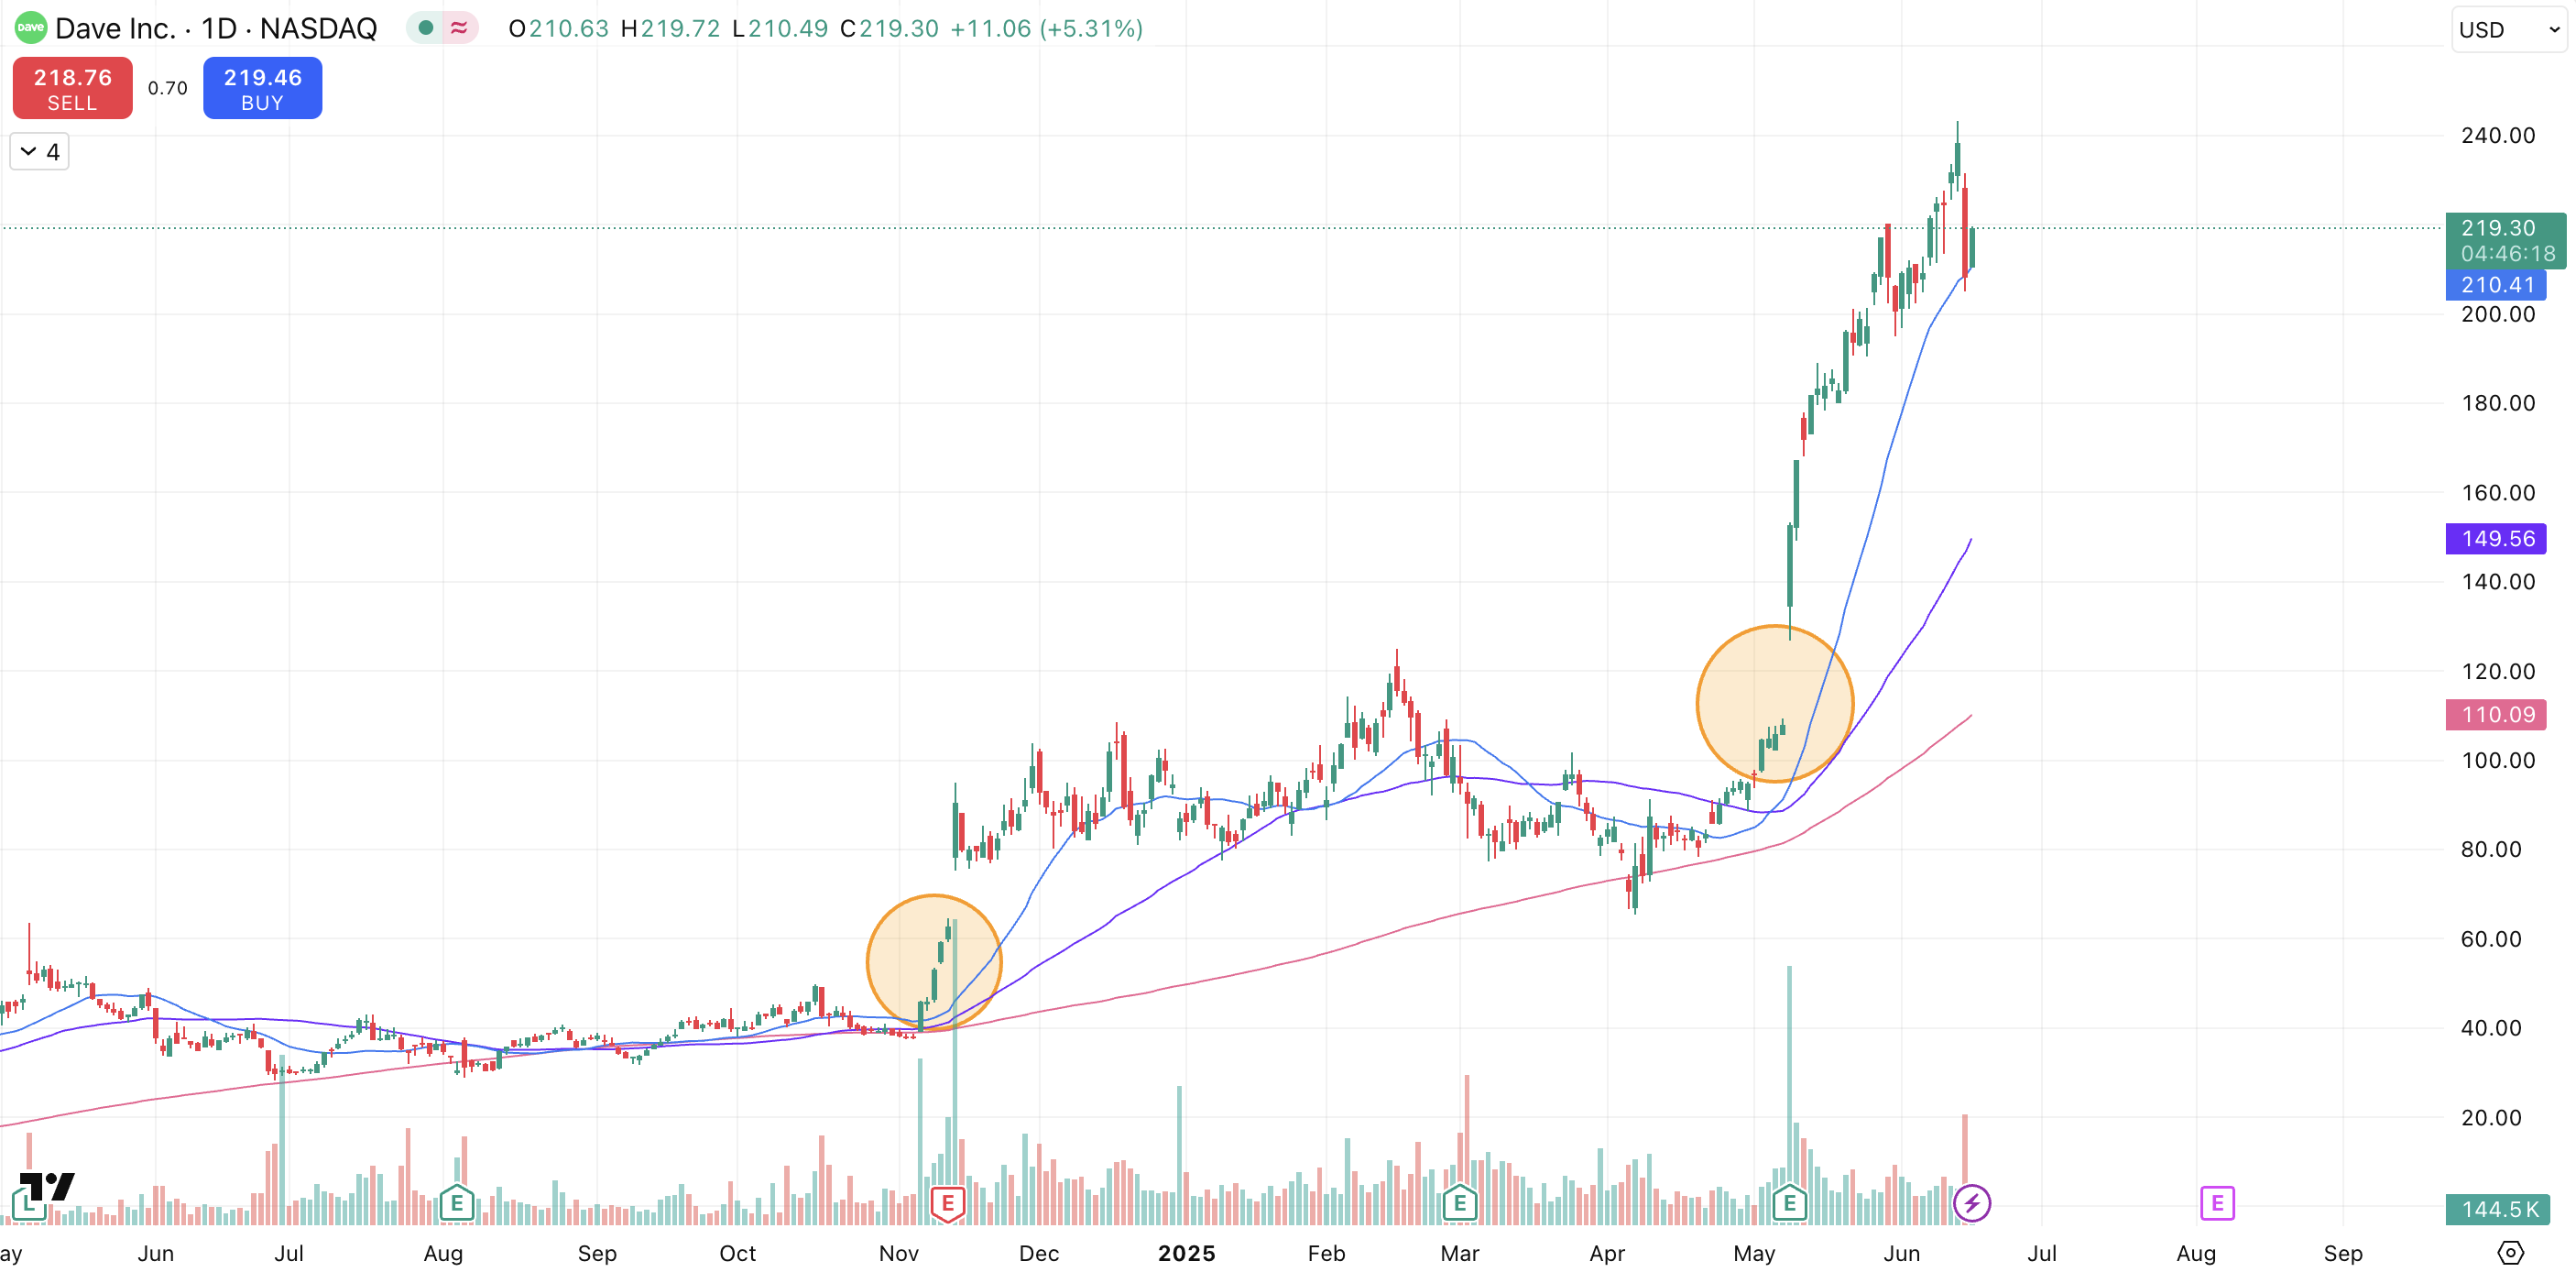
\includegraphics[width=0.8\linewidth]{images/DAVE2.png}
                \caption{Spike!}
            \end{figure}
        \end{itemize}
    \subsection{Pattern}
        Dave’s post-earnings spikes follow a clear pattern: thin float and high short interest set the stage, but the stock only erupts when there's a surprise narrative shift—like swinging to profitability, raising guidance, or removing a major overhang. Large beats on cash flow and EBITDA, coupled with strategic catalysts, trigger multi-day short squeezes. Without a fresh surprise or new catalyst, even strong results are largely ignored.
\end{document}
